\chapter{Background}
\label{chap:background}

In this chapter, pointers to and clusters of recent work in the fields relevant to the thesis, especially where they intersect, are presented. These give a sense of where the thesis is coming from, and what lead to the explorations made later on.


\section{Taking inspiration from psychology}
\label{sec:SA_foundation_and_basis}

\textbf{Self awareness (SA) in psychology:} \nl	

The notion and idea of \textit{self awareness} has been of great interest to humans throughout history. And despite its sometimes abstract and elusive nature, many thinkers (like e.g. psychologists and philosophers) have previously tried to give an explanation and description of this phenomenon or capability, primarily as observed in individual humans and animals. One has also tried to extend these descriptions and developed concepts to explain collectives consisting of individuals. A good survey of such descriptions and explanations regarding Self-Awareness in Psychology is given in some recent books on Self-Aware Computing Systems \cite{sacs16_ch2, sacs17_ch3} by P. R. Lewis et al, and will be used as a basis for this section and essay.

The notion of self awareness might give associations to other psychological terms like perception and consciousness, and we will look at some relationships these have with the main notion here of self awareness, in the psychological and (briefly) philosophical literature.
\newline

What exactly is self awareness? Is it \textit{awareness} of a \textit{self}? If so, this leads to the question: what constitutes a \textit{self}? And also, what does really \textit{awareness} mean? Some answers given in psychological literature, and in later time taken inspiration from into computer science, will now be explored.
\newline

	\subsection{Awareness}

	Before Lewis et al. \cite{sacs16_ch2} inclusively and succinctly introduces the concepts and interpretations relating to Self-Awareness, as they pertain to the psychological literature especially, they start off by giving the definition of \textit{awareness} by The \textit{Oxford English Dictionary}, which is "knowledge or perception of a situation or fact." Hence (by simply adding the prefix \textit{self}), "situational or factual knowledge/perception about a \textit{self}" might seem to be a reasonable first intuition of the notion of Self-Awareness. We will now discuss further what might constitute a so-called \textit{self}.


	\subsection{The \textit{Self}}

	Prominent western philosophers, like David Hume and Immanuel Kant, had some differing views on what constitutes a \textit{self} — although both might seem reasonable and relevant. 

	As Lewis et al. describes it \cite{sacs16_ch2}, Hume is known for postulating that all human knowledge is induced from experience. This then means for Hume that the \textit{self} is no concrete and physical entity in the world, but rather the bundle of experiences or perceptions unique to an individual.

	On the other hand, for Kant, the scope of the self is significantly extended — as he argues for the self being an actual entity being the subject of experiences, which is common through space and time. This subject or \textit{self} then combines information from experiences with concepts in the mind, as well as with the imagination — as well as acting upon this combined knowledge.


	\subsection{Self-Aware Individuals}

	Given a Humean view of the self (as described above), one might then consider self awareness to consist of an individual's knowledge of its experiences. Whereas the Kantian view of the self yields a self awareness consisting of a distinct and physical individual subject to experiences, combining information from these experiences, concepts, and the imagination.

	Early appearing terms in the psychology literature, pertaining to Self-Awareness and notions of self — being reminiscent of these two differing views by Kant and Hume — are found in the distinction between the \textit{objective/explicit self}, and the \textit{subjective/implicit self}, firstly elucidated by W. James in 1890 \cite{principles_of_psychology_james}, and further expounded in detail by Duval \cite{duval1972theory}. Here, the \textit{implicit} self, often referred to as the self-as-subject, is the "me"-self, subject to experiences. The self awareness in this "me"-self then, according to Duval, is described as "\textit{a state of consciousness in which attention is focused on events external to the individual's consciousness, personal history, or body}" \cite{duval1972theory}. The \textit{explicit} self however, often said to be the "I"-self, describes a self-as-object which can be discerned, observed, and reasoned about in the world. This "I"-self then, according to Duval, has an objective self awareness described as being "\textit{focused exclusively upon the self and consequently the individual attends to his conscious state, his personal history, his body, or any other personal aspects of himself}" \cite{duval1972theory}.

	One well-known "self awareness-test", having been used to deem whether someone or something is self-aware or not, is the so-called \textit{mirror test}. This consists of observing an individual's capability (or lack thereof) of noticing or self-recognizing, in a mirror, a discreet change in their own appearance (that was caused by someone else typically, while they were not paying attention e.g.). The presence of such a capability is argued (e.g. by Asendorpf et al. \cite{asendorpf1996self}) to demonstrate the presence of a \textit{secondary representation} (a constructed conceptual model if you will) of oneself and the world (the primary representation being the real world). 

	Given that the ability to construct such a conceptual model of oneself is required in explicit self awareness, one could wonder whether passing this "mirror test" would then be satisfactory for someone or something (like a system) to be self-aware. Haikonen \cite{haikonen2007reflections} however demonstrated how easy it was for a not-too-sophisticated computing system to pass this test — and hence weakened the validity of this "mirror test" to definitively conclude whether someone or something was indeed self-aware or not.

	As should be more and more apparent, there has been — and still is — a lot of ongoing discussions about what should be considered self awareness, and what should not — as well as about all the different variants observed (by e.g. Morin \cite{morin2006levels}).

	Morin defined self awareness as different from, but building upon the previously mentioned consciousness (where this in some cases are deemed more "primitive" aspects of self awareness), in that "self awareness is the capacity to become the object of one's own attention." However, he doesn't deny the subjective aspect of the self-aware individual, in that he believes a self-aware organism to be one that "becomes aware that it is awake and actually experiencing specific mental events."

	The importance of including such a \textit{subjective} (perhaps more underlying and primitive) level of self awareness, lies in the realization that self-aware agents (being uniquely situated in the world, collecting unique data from their unique sensing-apparatus) \textbf{is} subjective in nature. As such, since possibly heterogenous agents might collect widely different data (due to their situation and sensing capabilities) from the same exact phenomenon, it is crucial that we know from which \textit{subject} the data we have originates from.

	Perhaps or perhaps not due to this, others would object to Morin's definition, and actually include this subjective and implicit (or in other words "perceptual (or pre-conceptual)", as Lewis et al. \cite{sacs16_ch2} put it) experience in their definition of self awareness — leading to self awareness and consciousness being overlapping concepts. This would also lead more complex and "full-stack" Self-Aware systems to being extensions of this simpler and more primitive level of Self-Awareness.


	\subsection{Public and Private Self-Awareness}
	\label{subsec:public_private_SA}

	The distinction, as discussed above, between the implicit/subjective and the explicit/objective self and corresponding self awareness has given rise to many further developments in this notion, as is presented by Lewis et al. \cite{sacs16_ch2}. However, these further developments separate this seeming distinction of \textit{private self awareness} (previously described as e.g. personal, historical, and bodily knowledge regarding the self-as-object) and \textit{public self awareness} (previously described as awake, subjective, and unique experiences external to the self) a bit differently.

	Rather than the above notions of public and private self awareness, \textbf{private self awareness} instead here refers to the obtaining of "knowledge of internal phenomena, typically externally unobservable and accessible only to the individual" \cite{sacs16_ch2}. On the other hand, \textbf{public self awareness} now concerns the gathering of knowledge based on phenomena external to the self. If we choose to look at public self awareness in the implicit/subjective form, we have a "minimally" self-aware individual who is merely able to perceive (subjectively) the external environment in which it is situated. Conversely, we could also have a publicly self-aware individual in the explicit/objective form — which would be more concerned with public appearance, and how the individual is perceived in its in environment (e.g. by other individuals, in social settings). These definitions of private and public self awareness will be used from now on.


	\subsection{Levels of Self-Awareness}
	\label{subsec:SA_levels}

	There is large consensus about, due to the many degrees or variations to which an individual can be self-aware, that self awareness is not \textit{binary} or singular — but rather on a spectrum. As Lewis et al. highlights (\cite{sacs16_ch2, sacs17_ch3}), varieties of an individual's self awareness capabilities are often associated or characterized with one or more levels of self awareness. As such, several have attempted at defining such self awareness levels.

	One such definition, being comparatively broad and wide (to other similar treatments), containing 5 increasingly complex self awareness levels, is given by Neisser \cite{neisser1997roots}:

	\begin{enumerate}
		\item \textbf{Ecological self}
		
		The ecological self is the most minimal form of self awareness. It permits sufficient knowledge only for basic stimulus-response behaviour, as the individual has a basic awareness of stimuli. The ecological self can be thought of as the minimum requirement for the individual to not be unconscious.
		\item \textbf{Interpersonal self}
		
		The interpersonal self enables the individual to possess a simple awareness of its external interactions, permitting limited adaptation to others in the performance of tasks.
		\item \textbf{Extended self}
		
		The extended self extends the interpersonal self to permit reflection of interactions over time. The individual is aware of the existence of past and future interactions.
		\item \textbf{Private self}
		
		The private self allows the individual to process more advanced information concerning itself, such as thoughts, feelings and intentions.
		
		\item \textbf{Conceptual self}
		
		The conceptual self, or self-concept, is the most advanced form of self awareness, representing that the individual is capable of constructing and reasoning about an abstract representation of itself.
	\end{enumerate}

	This final level, the \textbf{Conceptual self}, is very much connected to the much-discussed term of \textit{meta-self awareness}. Meta-self awareness refers to the awareness of someone that they themselves are self-aware. This includes reasoning about its own self awareness, and is argued to be necessary (at least in humans) in order to adapt to changes, and to direct ones attention where it is needed — and that without it, thoughtlessness would ensue.

	We will see later on in Section \ref{sec:design_describe_sa_comp_systems} how these levels come into play in a fundamental basis and a proposed reference framework, for describing Computational Self-Awareness.


	\subsection{Self-Aware Collectives}
	\label{subsec:collective_SA}

	In her comparison of three distributed and collective biological systems (the brain, the immune system, and ant colonies), Mitchell \cite{mitchell_decentralizedSA} elucidates how — not only individuals, as has been the case until now, but — also collectives (consisting of individuals) can exhibit apparent global self awareness properties/capabilities. As she goes on to explain and make her case, she further elucidates how these apparent self awareness properties are only seen globally — but not in individuals (which in this case are neurons, ants, or lymphocytes - also known as white blood cells). The explanation for this, she proposes, is due to the distributed and statistical nature of this apparent self awareness. Through the many individual interactions in the collective — self awareness gets built up \textit{bottom-up}, and then gets fed back down to the lower-level components in a \textit{top-down}-fashion.

	Given that this apparent self awareness then was not present in the collective's individual components, but in the global collective, as a result of the many interactions of the lower-level components — we might say that the collectives exhibit \textbf{\textit{emergent}} self awareness.

	Hence, we can both analyse and describe Self-Awareness capabilities in individuals, as well as collectives of individuals.


	\subsection{Self-Expression}
	\label{subsec:SE}
	
	Lewis et al. \cite{sacs16_ch2} argues that self awareness properties alone (i.e. the ability to continuously acquire, update, and synthesise the self's models and knowledge about itself and its experiences) is of limited value, unless it is accompanied by associated behaviour. As Chandra et al. \cite{sacs16_ch4} argue, later on in the same book — if the self only takes data in, but does not use that data to do anything, then it is essentially a "data-sink". Hence, the accompanying notion of \textit{self-expression} is introduced as "behaviour based on self awareness" \cite{sacs16_ch2}. This behaviour could be highly dynamic (e.g. enabling self-adaptation, self-reconfiguration, self-explanation), as well as constituting a more "standard" system behaviour, where self awareness is not considered at all.

% --- \section END. ---



\section{Self-Awareness in already-existing Computing Systems}

	\subsection{SA-related Computing Systems}
	
		\subsubsection{Self adaptive systems}
		Run-time adaptation in Computing and Engineering systems is not a new thing, and this has been of interest across a range of research communities for quite some time \cite{sacs16_ch4}. The reason for this becomes apparent when one considers the problem of tackle unforeseen (at least at design-time) operational changes that can occur during run-time (like e.g. faults).

		An agent — in the context of computing systems — can be said to be a computing system situated in an environment (which it can perceive), having some goals, and possible actions it can perform (through actuators) to reach its goals. It can also be informed by some knowledge, and/or directly the signals it gets from its sensors.

		Especially within the engineering of \textbf{Self-adaptive} Systems and Intelligent Agents, such agents are often designed with properties which can be called Self-Awareness and -Expression properties — even though these specific terms are not used.

		Notable examples in accordance with the autonomic computing paradigm (\cite{sacs16_ch4}) comprise for example ODA (Observe-Decide-Act) loops, originally stemming from the OODA (Observe-Orient-Decide-Act) loop in the military domain. As the acronym suggests, systems implementing the ODA-loop continually Observe (their environment and potentially themselves through sensors), Decide (planned future actions based on current or future states), as well as Act (on one of those previously planned actions). A schematic of such an ODA-loop can be seen in Figure \ref{fig:oda_mapek}.

		\begin{figure}[ht]
		\centering
		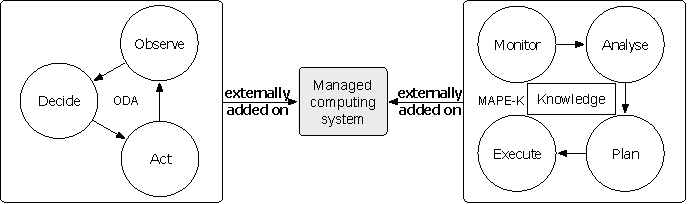
\includegraphics[width=\columnwidth]{Assets/DocSegments/Chapters/Background/Figures/Schema/oda_mapek.pdf}
		\caption[Previous and prevalent computational self adaptive agent frameworks.]{Figure of the Self-adaptive Systems ODA (left) and MAPE-K (right). We also see the externality of the attempts at implementing meta-self awareness in these systems, in that they simply \textit{add on} an external Managed computing system (which is monitoring the rest of the system). Figure reused from Chandra et al. \cite{sacs16_ch4}.}
		\label{fig:oda_mapek}
		\end{figure}

		Another notable Self-adaptive System we can see in Figure \ref{fig:oda_mapek}, is the MAPE-K architecture (an acronym for Monitor, Analyse, Plan, Execute, and Knowledge). The great and groundbreaking benefits of implementing e.g. ODA-loops and the MAPE-K architecture, performing online observation and knowledge-gathering (hence having endowed their systems with some sort of self-knowledge/self awareness) allowing for online self-adaptation — have been greatly reaped. However, these architectures have not explicitly considered the psychological origins of self awareness, and lack some benefits compared to the introduced frameworks and architecture in Section \ref{sec:design_describe_sa_comp_systems}.
	
	
		\subsubsection{Music technology systems and musical robots}
		\label{music_tech_robots}

		As particularly relevant to the thesis project, endowing Music Technology Systems with Self-Awareness is of great interest. There have been several such approaches, particularly within Interactive and Active Music Systems. One example includes:

			\paragraph{SoloJam: Achieving de-centralized participation (by co-ordinating and co-operating agents) in a coherent and interactive music system \nl}

			Historically, the creation and production together with the listening and perception of music has been (and still is) relatively "one-way'ed"; in that the musicians/artists produce the music, and the fans/listeners consumes the music. A growing interest in interactive music (like Guitar Hero etc.) has been seen the last decades. The authors of the music system SoloJam \cite{solojam} want participants with little or no musical experience and training to be able to play independently and decentralized (from say an expert) music as a whole, by each playing solos made from their own devices. Here each of their solos will be slight variations of the previous participant's solo. See illustration in Figure \ref{fig:solojam}.

			\begin{figure}[!htp]
			\centering
				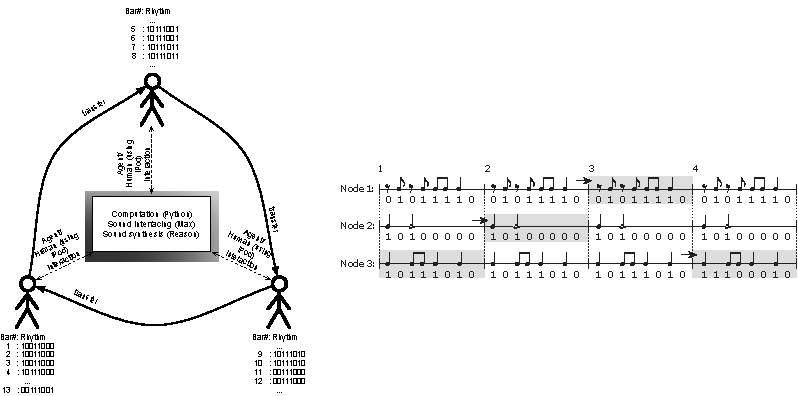
\includegraphics[width=\columnwidth]{Assets/DocSegments/Chapters/Background/Figures/Schema/SoloJam.pdf}
				\caption{Illustrations: two individual SoloJam example scenarios illustrated differently.}
				\label{fig:solojam}
			\end{figure}

			The solution to how this decentralized, coherent and interactive music system consist of elements inspired by the Economical Sciences. Namely:

			\begin{enumerate}
				\item Auctions (specifically the Vickrey auction)
				\item Utility (profitability/deservedness measure)
			\end{enumerate}

			The function for utility is given by the expression:

			\begin{equation}
			u_i = \frac{c}{(1+a D_l)(1+b T_l)}
			\end{equation}
			\newline

			It is essential with a properly designed utility function for the system to behave coherently e.g. This utility-function is inversely proportional with \textit{a)} differences between bidder and auctioneer's/leader's rhythm patterns $D_l$, and \textit{b)} the time/\#bars the leader has played its rhythm pattern $T_l$ - as well as constrained by and applied to a couple of other clauses (to ensure some wanted/avoid some unwanted effects).

			"Shaking"-/"moving"-patterns (as registered/sensed by the devices' inertial units) are translated into rhythm patterns - which then are calculated a \textbf{utility score} (by the function as mentioned above and outlined in more detail in the paper) for, used as bid in an auction.

			The winner of the auction will (when considering knowledge of the leader-rhythm-pattern, as we do when a = 1.0 instead of 0.0) be those rhythm patterns which are the closest rhythm-patterns (i.e. not completely equal) to the leader's rhythm-pattern (in terms of the Hammings-distance) - assuming e.g. that the participant didn't just play before another participant, nor that it had played its rhythm-pattern for a very long time. In the paper, we then notice how the authors study how \textbf{varying degrees of self awareness} (a=1.0 versus a=0.0) affect the overall system dynamics — then in the form of musical coherence, as well as decentralized circulation.

			
			\paragraph{Musical robots: the Dr. Squiggles \nl}
			\label{dr_squiggles}
			
			The Dr. Squiggles robots, which are M. J. Krzyzaniak and RITMO's musical robots, as e.g. can be seen in Figure \ref{fig:background_dr_squiggles_synchronizing} as they synchronize to each other, have been used in several music technology systems and projects\footnote{\url{https://www.uio.no/ritmo/english/news-and-events/news/2021/drsquiggles.html} (accessed 2022.05.17)} previously.
			
			\begin{figure}[!htp]
			\centering
				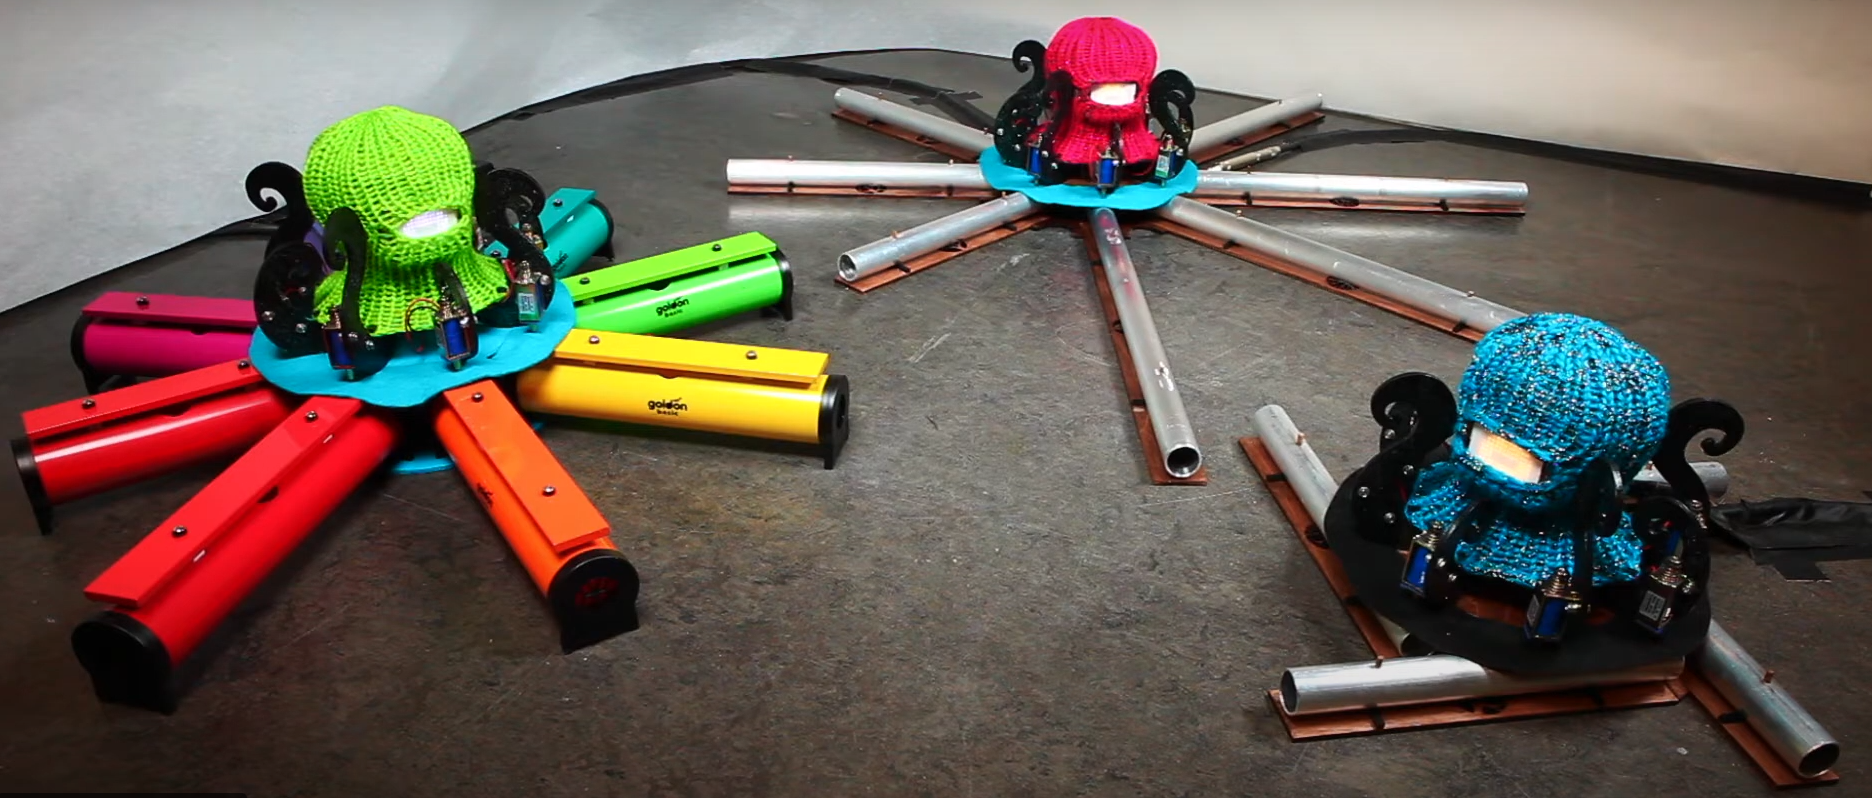
\includegraphics[width=\columnwidth]{Assets/DocSegments/Chapters/Background/Figures/Photos/dr_squiggles_synchronizing.png}
				\caption[Three Dr. Squiggles robots synchronizing to each other.]{Three Dr. Squiggles robots synchronizing to each other. Photo: from M. J. Krzyzaniak's video \textit{Squiggles Equilibrium}\protect\footnotemark}
				\label{fig:background_dr_squiggles_synchronizing}
			\end{figure}
			\footnotetext{\url{https://www.youtube.com/watch?v=yN711HXPfuY} (accessed 2022.05.27)}
			
			
			\paragraph{SoloJam Island \nl}
			\label{solojam_island}
			
			Combining the two musical systems presented above, Pierre Potel implemented islands of Dr. Squiggles robots in a SoloJam scenario, and hence naming the novel musical robot system \textit{SoloJam-Island}\footnote{\url{https://github.com/67K-You/SoloJam-Island} (accessed 2022.05.17)}. Corresponding 3D-models of the Dr. Squiggle robots, for said simulation, were designed by Pierre Potel.
			

	\subsection{Explicit self awareness in computing systems}
	The extensive interest of studying self awareness in natural fields like psychology, sociology, and philosophy might not come as a surprise, as self awareness primarily is found and exhibited in humans and animals. However, there has recently been an uptake in interest for explicitly studying self awareness in computing systems.

	Recently, (often collaborative) efforts within the computer science \& engineering community \cite{sacs16_ch2, sacs17_ch1, sacs17_ch3} have lead to a greater systematic understanding of self awareness, and how it can be used and evaluated within Computing Systems.

	Some of these fields, now explicitly interacting with the notion of self awareness — as they were presented in overviews given by P. R. Lewis et al. \cite{sacs17_ch3} and S. Kounev et al. \cite{sacs17_ch1} — includeautonomic computing, machine learning and artificial intelligence, multi-agent systems, self-organizing and self-adaptive systems, situation-and context-aware systems, reflective computing, model-predictive control, as well as work from the models@run-time community. But also, fields like Robotics, complex IT systems, computer engineering, and reflective architecturing \cite{sacs17_ch3}.

	Some quite notable research projects and initiatives within computer science and engineering, explicitly engaged with the notion of self awareness in computing has been performed (like the SEEC project at MIT and University of Chicago, the ASCENS and EAssets/pics FP7 EU Projects, as well as the SEAMS Dagstuhl Seminars and workshop series) \cite{sacs17_ch1}.


		\subsubsection{Specific Examples}

			\paragraph{Cognitive Radios \nl}

			A — perhaps simpler or minimal — specific instance of a computing system where Self-awareness have been interpreted and applied, is the so-called \textit{cognitive radio}. The devices in this system control their own capabilities and monitor other devices' capabilities through communication with these other devices. This "\textit{enables them to improve the efficiency of communication by negotiating changes in parameter settings}" \cite{sacs17_ch3}

			\paragraph{CoCoRo: the self aware underwater AUV swarm \nl}

			More complex self-aware computing systems have also been explored. As demonstrated by Mitchell \cite{mitchell_decentralizedSA}, also T. Schmickl et al. considers self awareness in a collective system — an underwater swarm robotic system \cite{cocoro} in this case (see Figure \ref{fig:cocoro}). This robot collective shall in this scenario search the sea-bottom for specific objects of interest (like toxic waste, but also sunken objects e.g.). Here, the collective/swarm is supposed to e.g. be self-aware of its own state (of whether it still is searching, or if it has found a target at the bottom of the sea) — in order to either stay together searching, or communicate to a second (surface level) swarm that an object of interest is found. Like in Mitchell's case, these autonomous underwater vehicles (AUVs) does have emergent self awareness properties that the individuals themselves do not possess. Therefore, as the authors say in \cite{cocoro}, "\textit{Finding such targets will only be efficient if the AUVs work together}."

			\begin{figure}[!ht]
			\centering
			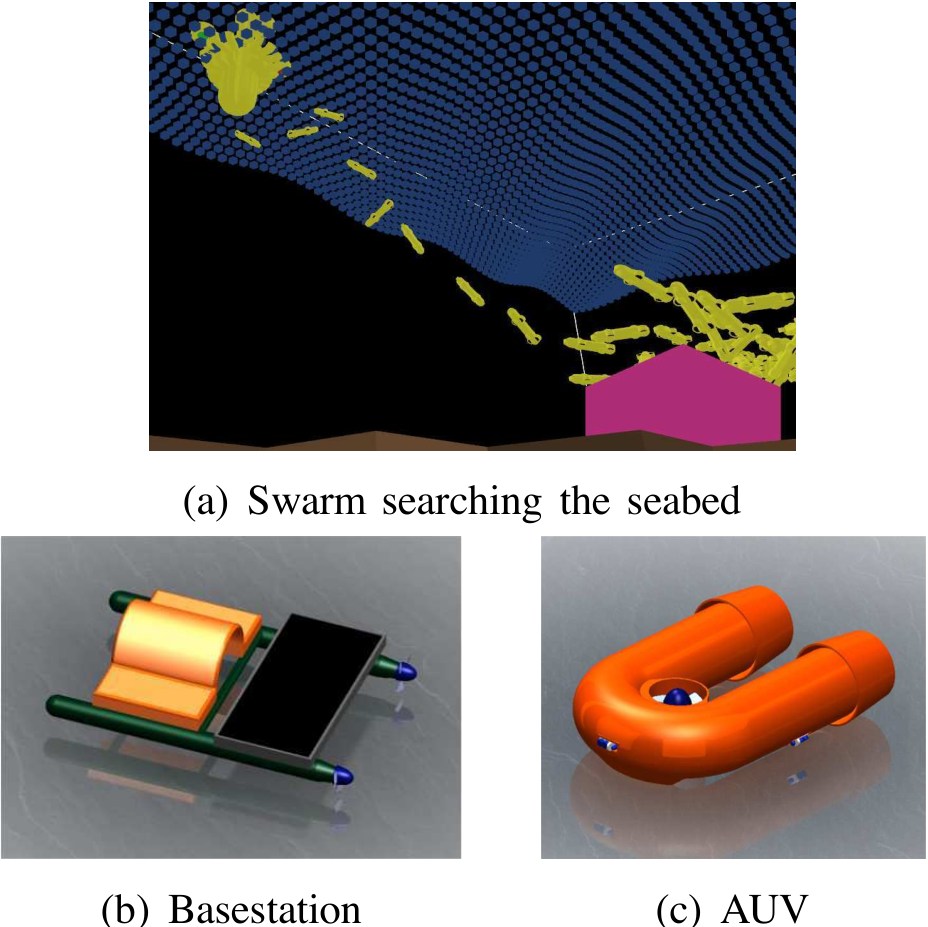
\includegraphics[width=0.65\columnwidth]{Assets/DocSegments/Chapters/Background/Figures/Schema/cocoro.PNG}
			\caption[CoCoRo: the self aware underwater robotic AUV swarm.]{CoCoRo: the self aware underwater robotic swarm consisting of AUVs alternating between completing missions at the seabed and returning to the surface level basestation. Figure reused from T. Schmickl et al.'s paper \cite{cocoro}.}
			\label{fig:cocoro}
			\end{figure}

			\paragraph{Self-Aware and Self-Expressive Camera Networks \nl}

			Lukas Esterle et al. \cite{sa_and_se_camera_networks} has demonstrated how the fundamental concepts and building blocks of Computational Self-Awareness and Self-Expression can handle resource-critical- as well as communication- and utility-tradeoffs, maintaining network topologies, performing distributed object detection, performing tracking handover, as well as achieving more Pareto-efficient outcomes. They also believe these capabilities are not exclusive to camera networks — but are in fact confident these technologies (of computational SA and SE) can enable "\textit{other types of systems and networks to meet a multitude of requirements with respect to functionality, flexibility, performance, resource usage, costs, reliability, and safety}" \cite{sa_and_se_camera_networks}.
			
% --- \section END. ---



\section{Designing and Describing Self-Aware Computing Systems}
\label{sec:design_describe_sa_comp_systems}

Psychology has served as the basis \& main source of inspiration. Here we will look at a translation of Self-Awareness, from Psychology to Computing. We will hence look at an introduction of the new notion of \textit{Computational Self-Awareness}.

Translating concepts from the Psychological field into the Computational field gives rise to rich sources of inspirations (for engineers and researchers who might not have thought psychologically about designing and describing computing systems), as well as hopefully clear, structured, principled conceptual tools to in a consistent manner describe and design so-called \textit{Self-Aware Computing Systems}.

	\subsection{Basis and Fundament}

	Lewis et al. \cite{sacs16_ch2} have introduced a basis and fundament for Computational Self-awareness and Self-expression, that is founded in the psychological literature on Self-Awareness, as presented in Section \ref{sec:SA_foundation_and_basis}.

	More specifically, they base their new notion of computational self awareness on computationally translated versions of the key self awareness concepts discussed in Subsections \ref{subsec:public_private_SA}, \ref{subsec:SA_levels}, and \ref{subsec:collective_SA}, as well as \ref{subsec:SE}.

	First off, public and private self awareness now considers computational systems, instead of human selves — but these definitions are still the same (only that now the \textit{self} is the \textit{computational system}).

	Secondly, Neisser's five levels of self awareness is now translated by P. Lewis et al. \cite{sacs16_ch2} into five corresponding levels, as shown in Figure \ref{fig:comp_SA_levels} below.

	\begin{figure}[!htp]
		\centering
		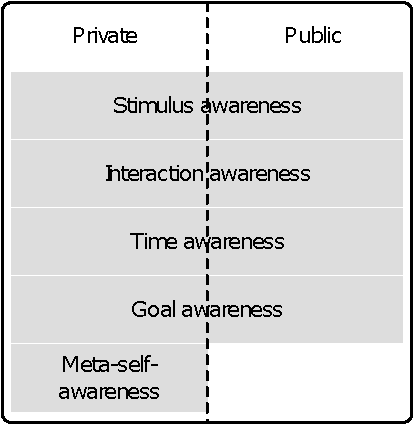
\includegraphics[width=0.5\columnwidth]{Assets/DocSegments/Chapters/Background/Figures/Schema/SA_levels.pdf}
		\caption[Translated levels of self awareness from psychology to computer engineering and robotics.]{Translated levels of self awareness from psychology to computer engineering and robotics. Figure credits: Lewis et al. \cite{sacs16_ch2}.}
		\label{fig:comp_SA_levels}
	\end{figure}

	Thirdly, computational self awareness can both be considered in individual agents/computing systems, or in arbitrary agent-collectives (consisting of several sub-collectives) — as seen in \ref{fig:collective_SA} below.

	\begin{figure}[!htp]
		\centering
		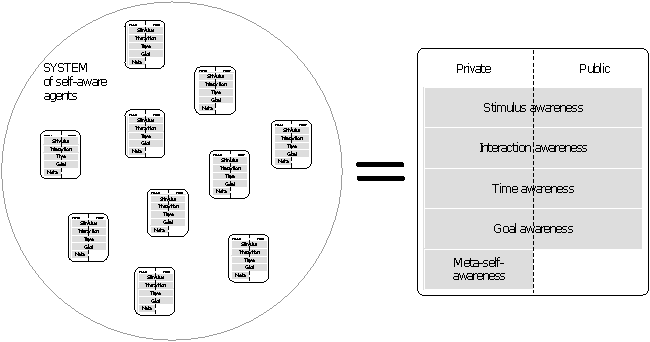
\includegraphics[width=\columnwidth]{Assets/DocSegments/Chapters/Background/Figures/Schema/collective_SA.pdf}
		\caption[Collective self awareness schema.]{Collective self awareness schema, as entities can be seen as consisting of many sub-entities. Figure credits: Lewis et al. \cite{sacs16_ch2}.}
		\label{fig:collective_SA}
	\end{figure}

	Lastly, \textit{Computational Self-Expression} is similarly defined as  (only now for a computing system as the \textit{self}) \textbf{behaviour based on \textit{computational} self awareness}.
	\newline

	Kounev \& Lewis et al. also gives a definition of Self-aware Computing \cite{sacs17_ch1}:

	\textbf{Definition 1.1} Self-aware computing systems are computing systems that:

	1. \textit{learn models} capturing \textit{knowledge} about themselves and their environment (such as their structure, design, state, possible actions, and runtime behavior) on an ongoing basis and

	2. \textit{reason} using the models (e.g., predict, analyze, consider, and plan) enabling them to \textit{act} based on their knowledge and reasoning (e.g., explore, explain, report, suggest, self-adapt, or impact their environment)

	— in accordance with \textit{higher-level goals}, which may also be subject to change.


	\subsection{Reference Architecture}

	Chandra et al. introduces their own new Reference Architecture for designing and describing Computational Self-Awareness and Self-Expression \cite{sacs16_ch4}. This abstract and conceptual framework has several advantages. Firstly, it provides a detailed and fine-grained separation of different self awareness and self-expression processes — and hence makes design- and engineering-questions easier and more methodical. Secondly, being a common language, it paves the way for identifying common architectural patterns used to design Comp. SA- \& SE-systems. Compared to other Self-Adaptive systems, it also includes the notions of Self-Awareness from the beginning (as the psychology literature suggests SA capabilities is more innate than simply an add-on). And due to the general and implementation-agnostic framework, it can be used on a wide variety of agents systems, or agent-collectives systems.

	A schematic of this reference architecture is given below:

	\begin{figure}[!htp]
		\centering
		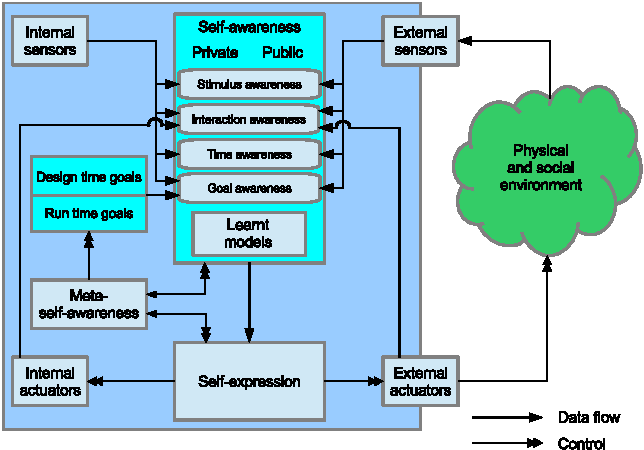
\includegraphics[width=0.9\columnwidth]{Assets/DocSegments/Chapters/Background/Figures/Schema/SA_and_SE_architecture.pdf}
		\caption[A rererence architecture for a self aware, and self expressive, computing system.]{Chandra et al.'s \cite{sacs16_ch4} rererence architecture for a self aware, and self expressive, computing system. Figure credits: Lewis et al. \cite{sacs16_ch4}.}
	\end{figure}


	\subsection{Conceptual Framework}

	Lewis et al. \cite{sacs17_ch3} introduces an inclusive and extensive Conceptual Framework, built and based on the psychological foundation and basis \textit{(as well as expanding on the Reference Architecture)}, as introduced earlier in this section.

	This Conceptual Framework is based on the following three high-level concepts/tenets:
	\begin{enumerate}
		\item \textbf{Levels} of self awareness
		\begin{itemize}
			\item \textbf{Pre-Reflective self awareness} — ability to subjectively and uniquely perceive and experience phenomena in the physical-/social-environment as well as within itself. A pre-requisite for all other and more advanced forms of computational self awareness, also implicitly introducing the notion of subjectivity.
			\item \textbf{Reflective self awareness} — modelling and conceptualizing various knowledge-/awareness-aspects about an \textit{object}, where the object is what is modelled, or the sensory observation of it at least.
			\item \textbf{Meta-Reflective self awareness} — \textbf{Reflective self awareness} processes about its own self awareness processes. Reasoning and modelling of the oneself's own (as well as potentially other systems') self awareness properties and processes. Typically its \textit{objects} are 1) the self awareness (modelling) processes themselves, and 2) the output of these processes, i.e. the models themselves. And often the combination (e.g. the memory usage of the learning of an AI model, versus the accuracy of the model — hence potentially calling for a change in architecture or algorithm-choice in a self awareness process) are useful.
		\end{itemize}
		
		\item \textbf{Aspects} of Reflective and Meta-reflective Self-awareness
			\begin{itemize}
				\item All the different aspects and facets of models being learnt and reflected with (like temporal aspects, interactive/causing, identity and state aspects, behavior awareness, appearance awareness, goal awareness, belief awareness capturing uncertainty and trust-levels, expectation awareness combining belief- and time-awareness).
				\item Not a comprehensive and large list of requirements a system has to check off in order to be considered Self-Aware (due to specific context or system design situations calling for different needs) — but rather a good starting point for considering the aspects captured in reflective and meta-reflective self awareness.
			\end{itemize}
			
		\item \textbf{Domain} of Self-awareness, being the combination of the two;
			\begin{itemize}
				\item Span (subject(s) of reflective self awareness, comprising all entities that contribute to the formation of self awareness)
				\item Scope (object(s) of self awareness, comprising all the entities observed by the subject's self awareness). E.g., in the case of robotics, the number or amount of neighbouring robots they are aware of and communicate with.
			\end{itemize}
	\end{enumerate}

	From \cite{sacs17_ch3}:

	"\textit{Using the intersection of all three tenets, we may produce descriptions of the
	specific self awareness of a system. For example, we might construct a sentence as
	follows: Peter (span) is aware of Ada’s (scope) goal (aspect) to reduce the power usage
	(object). Further, Ada (span) is aware of her own reasoning (meta-self awareness) about what to do (act) about it.}"


	\subsection{Challenges \& Limitations}

	Physical constraints like computational processing power, as well as time, limited attention e.g. are all significant constraints which designers of Self-Aware and Self-Expressive Computing Systems have to keep in mind.

% --- \section END. ---



\section{Taking inspiration from natural phenomena}
The intriguing, diverse, and complex phenomena of nature have for long served as exciting inspirations to human engineers and researchers [ant-colonies, boids, swarms, beeclust].

Often times, scientists have drawn inspiration from various scientific fields — particularly different fields from ones own — into their own field, for various reasons. Indeed, the translated concepts (from the one domain to the other) will most likely be accompanied with brand new ways to think about ones own domain, as well as other domains again interacting with it (hence having a real opportunity to start a "domino"-like chain-reaction of new ways to think about things emerging). These new ways to think about things (often in ones own domain) — apart from being interesting and intriguing — might be useful, both for ones own field but also for other fields again (especially if thinking long term). For example in the Multi-Agent Systems (MAS) field, it has been a common practice to study complex biological systems in nature, in order to translate these mechanisms into the technology- and engineering-domain. Such bio-inspired algorithms have been some of the most widely used optimization algorithms throughout history, with e.g. the original paper by M. Dorigo et al. for the ant colony optimization algorithm \cite{dorigo_ant_2006}, as of May 2022, having 14 743 citations on Google Scholar. Another example is how D. Goldman et al. \cite{sandbots} took inspiration from e.g. zebra-tailed lizards able to run up to 5 meters per second (normally in desert sand) when designing a robot traversing one of the most challenging terrains to traverse through, granular surfaces like sand that is. Natural phenomena have then been subject to considerable study and modelling—and have in fact created entire scientific fields in which principles from various science- \& engineering-dicipline are applied to the physical systems and machines having functions that mimic biological processes, as well as biological processes serving as great sources of inspiration for the engineered systems; \textit{Biomimetics}\footnote{\textit{Nature}, \url{https://www.nature.com/subjects/biomimetics} (accessed 2022.05.17)} and \textit{Bionics}, that is.

One branch of these types of natural phenomena observed and studied are the biological networks of pulse-coupled oscillators \cite{proskurnikov_synchronization_2016, neda2000selfsorganizing}. An example of such biological pulse-coupled oscillators as found in nature, particularly of interest for this thesis, is the synchronously flashing fireflies, as e.g. can be seen in a dark forest in Figure \ref{fig:synched_fireflies_phenomenon} in Chapter \ref{chap:introduction}. This phenomenon has inspired scientists like e.g. Mirollo \& Strogatz \cite{mirollo_strogatz_PCO_synch} and in later time Kristian Nymoen et al. \cite{nymoen_synch}, to model and replicate this natural phenomenon in human-engineered systems. Given the periodic and repeating nature of the flashing/firing of the fireflies, modelling a firefly has been done by looking at each firefly as a periodic signal or oscillator. This work \cite{mirollo_strogatz_PCO_synch, nymoen_synch} then ties into the broader work on synchronizing oscillators which has been subject to study for some time now []. What separates Mirollo-Strogatz and K. Nymoen's approaches from these other and previous oscillator-synchronizing methods, is mainly that here the oscillators are \textit{pulse-coupled} (which the fireflies also can be said to be), as opposed to the more ``standard'' and constraining \textit{phase-coupled} oscillators. Additionally, K. Nymoen's approach accounts for synchronizing initially heterogenous frequencies as well.

% --- \section END. ---



\section{Oscillators and oscillator-synchronization}


	% --- META INFO START: ---

	\gjor{ Beskriv dette så godt at du kan snakke fritt om oscillatorers \textbf{faser} og \textbf{frekvenser} senere (i Implementation f.eks.), spesielt i tilfelle for noen ikke har vært borti det før, eller tatt et Signalbehandlings-kurs }

	\gjor{ Skill på Pulse-coupled Oscillators, og Phase-coupled Oscillators. Nevn fordelene, spesielt for roboter, med å synkronisere seg basert på diskret tid [Sandsbots-paperet Kyrre sendte deg (iaff. slutt-tabellen), SandBots-arkitekturen som åpner for lave oppdaterings-rater], sammenliknet med kontinuerlig tid }

	\besk{ Teori og nyere cutting-edge/state-of-the-art metoder for fase-/frekvens-synkronisering i oscillatorer og liknende. Se Kristian Nymoens referanser \cite{nymoen_synch} og artikler funnet i denne veinen } \nl

	% --- META INFO STOP. ---


Oscillators have been used to implement and model a plethora of systems, also biological ones, ranging from designing the locomotion-patterns of swimming robot-amphibia through central pattern generators \cite{ijspeert_cpg}, ..., and as we have already established, modelling synchronously flashing or firing fireflies.
	
	
	\subsection{Phase and frequency}
	Much of the terminology from \cite{nymoen_synch} is used here. An oscillator $i$ is characterized by its \textit{phase} $\phi_i(t)$, which is—at the start of its periodic signal period—initialized to 0 and evolves towards 1 at a rate which is called the \textit{frequency} of the oscillator. So, in mathematical terms, the frequency $\omega_i(t)$ is then given by:
	
	\begin{equation}
	\label{phase_freq}
		\omega_i(t) = \frac{d \phi_i(t)}{d t} .
	\end{equation}

	When oscillator $i$'s phase is equal to 1 (i.e. when $\phi_i(t)=1$, or when the periodic signal period is over), we say oscillator $i$ has \textit{phase-climaxed}.
	
	An oscillator-period $T$ is defined as the inverse of the oscillator-frequency $\omega$. In mathematical terms:
	
	\begin{equation}
	\label{period_freq}
		T = 1/\omega .
	\end{equation}
	
	
	\subsection{Phase synchronization}
	
		\subsubsection{Mirollo-Strogatz's ``standard'' phase adjustment} % or phase synchronization, or phase updates
		\label{mirollo_strogatz_phase_adjust}
		
		
		One approach having been used to achieve this in the past is Mirollo-Strogatz's ``Standard'' phase adjustment in oscillators \cite{mirollo_strogatz_PCO_synch}, as seen a sketch of in Figure \ref{fig:mirollo_strogatz_phase_adj_sketch}.
		
		\begin{figure}[ht!]
			\centering
			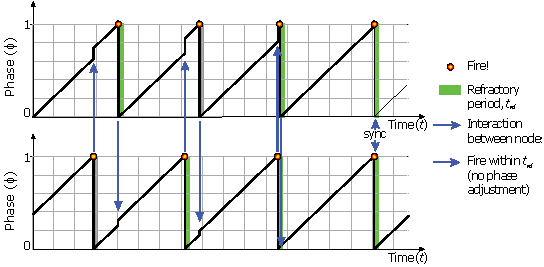
\includegraphics[width=\linewidth]{Assets/DocSegments/Chapters/Background/Figures/Illustrations/MirolloStrogatzPhaseSync.pdf}
			\caption[Sketch of Mirollo \& Strogatz's ``standard'' phase adjustment.]{A sketch of Mirollo \& Strogatz's ``standard'' phase adjustment. Figure credits: K. Nymoen et al. \cite{nymoen_synch}.}
			\label{fig:mirollo_strogatz_phase_adj_sketch}
		\end{figure}
		
		Each oscillator gets a new phase, $\phi(t^+) = P(\phi(t))$, accoring to the \textbf{phase update function \eqref{strog_phase}} upon perceiving a ``fire''-event from one of the other musical nodes:
		
		\begin{equation}
		\label{strog_phase}
			\phi(t^+) = P(\phi(t)) = (1 + \alpha)\phi(t) ,
		\end{equation} \nl
		where $\alpha$ is the pulse coupling constant, denoting the strength between nodes \cite{nymoen_synch}, $t^+$ denotes the time-step immediately after a ``fire''-event is heard, and $\phi(t)$ is the old frequency of the oscillator at time $t$. 
		
		So, if e.g. $\alpha = 0.1$, then a musical oscillator's new and updated phase, immediately after hearing a ``fire''-signal from another oscillator, will be equal to $\phi(t^+) = P(\phi(t)) = (1 + 0.1)\phi(t) = 1.1\phi(t)$. 110\% of its old phase $\phi(t)$, that is. Hence, and in this way, the oscillator would be ``pushed'' to fire sooner than it would otherwise (as nodes fire once they have reached phase-climax $\phi(t)=1$).
	
	
	\subsection{Frequency synchronization}
	
		% --- META INFO START: ---
	
		\besk{ \tcol[gray]{(If relevant and wanted)} Previous approaches to Frequency-synchronization in oscillators (pulse- and/or phase-coupled) [nymoen-referanser e.g.] where the oscillators's frequencies are either equal and fixed, or where frequencies are bound to initialize and stay within a fixed interval/range. }
		
		\besk{ \tcol[gray]{(If it exists)} A ``simpler'' frequency synchronization approach, to solve the phase and frequency ($\phi$ \& $\omega$) problem with, without any self awareness components }
	
		% --- META INFO STOP. ---
	
% --- \section END. ---